\documentclass{article}

\usepackage{arxiv}
\usepackage[ruled,vlined]{algorithm2e}
\usepackage[utf8]{inputenc}
\usepackage[T1]{fontenc}
\usepackage{url}
\usepackage{booktabs}
\usepackage{amsfonts}
\usepackage{nicefrac}
\usepackage{microtype}
\usepackage{graphicx}
\usepackage[font=small,labelfont=bf]{caption}
\usepackage{cite}
\usepackage{pdflscape}
\usepackage{listings}
\usepackage{outlines}


\title{DRAFT PROPOSAL - Logs lineage and tiered segments in Apache Kafka}

\begin{document}

\section{Objectives}
The purpose of this document is to describe how remote log segments (offloaded to a tiered storage and not available in brokers log directories) are handled to guarantee an access to data which provides agnosticity towards the storage tier.

\subsection{Lineage equivalence}

The functional behaviour proposed in this document boils down to one principle - to preserve lineage of replicas regardless of the storage tier where they are stored. This is required to reproduce the current behaviour of Apache Kafka for which log segments are always accessed locally.

Under \textit{lineage equivalence}, the current specifications in case of divergence of log lineage should be preserved, and no discrepancy should be introduced in the data a consumer would expect to find with or without tiered storage.

\subsection{Notations}
Consider a topic-partition. In this document, we will note $S_i^r$ the i-th segment of a replica $r \in AR$ and $[BO_i^r..EO_i^r]$ the range of offsets of $S_i^r$ from the base offset $BO_i^r$ to the end offset $EO_i^r$. The log end offset at epoch $k$ is referred to as $LEO_k$\footnote{$LEO[LG_K]$ in figures.}.

\section{Preservation of local replica lineage in case of diverging replicas partially or totally tiered}

One consequence of unclean leader election is a possible divergence of log lineages which can happen when leadership of a topic-partition is acquired by an out-of-sync replica. It is possible that a log segment which is offloaded (uploaded) to a tiered storage presents offset overlap or contains duplicated and/or divergent records with already tiered log segments.

\subsection{Simplified example}

Let us consider the following simplified example, in which a topic-partition is made of two replicas 1 and 2 on a cluster with tiered storage available and unclean leader election enabled. Figure \ref{fig:simple-example} illustrates the successive states and locations of the log segments under study.

\begin{outline}[enumerate]
	\1 At $t_1$, replica 1 is the leader and replica 2 is out of the ISR set. The segment $S_i^1$ has been rolled over, and $S_{i+1}^1$ is the active segment of replica 1. Since the ISR is reduced to the leader replica, the leader high watermark can progress to the log end offset $LEO_k$. Assume there is no transactional records, so that the log stable offset corresponds to the leader high watermark, and ahead of $EO_i^1$, so that segment $S_i^1$ is eligible for tiering. Assume the leader 1 offloads successfully $S_i^1$ which is mapped to the unique ID $u_k$. Assume that afterwards, that segment is locally deleted to honor the configured log retention policy.
	\1  At $t_2$, replica 1 becomes offline and replica 2, then only live replica of the topic-partition, is elected as the leader under application of the offline leader election strategy. Leader generation is incremented from $k$ to $k + 1$.
	\1  At $t_3$, replica 1 is back online and becomes a follower of replica 2. It attempts truncating its local log to $LEO_{k+1}$, which is outside of the range of offsets covered by the local segments. However, assume that (a) $LEO_{k+1} \in [BO_i^1..EO_i^1]$, thus within the range of offsets covered in the tiered storage. Also, note that by construction of this example, (b) the leader epoch of replica 1 before becoming follower is $k$. The follower 1 then decides to onload the segment with the key $u_k$.\footnote{We will see later on why these two conditions are important.} Truncation to $LEO_{k+1}$ then occurs as would have initially been for a local segment. In this example, this results in few diverging records, which were produced to $S_j^2$ but not replicated to $S(u_k)$.
	\1 At $t_4$, replica 2 ingested enough records for the segment $S_j^2$ to be rolled-over and tiered, assuming the necessary conditions are met. This results in two segments in the tiered storage with both duplicated and divergent records.
\end{outline}

The behaviour illustrated in this scenario is chosen so that data uniform access is enforced, that is to say, the lineage of replica 1 resulting from an unclean leader election needs to be exactly identical whether part of this lineage is remotely or locally available. In this example, a remote segment is onloaded to the log directory and reinstated as an active segment.

\begin{figure}[h!]
	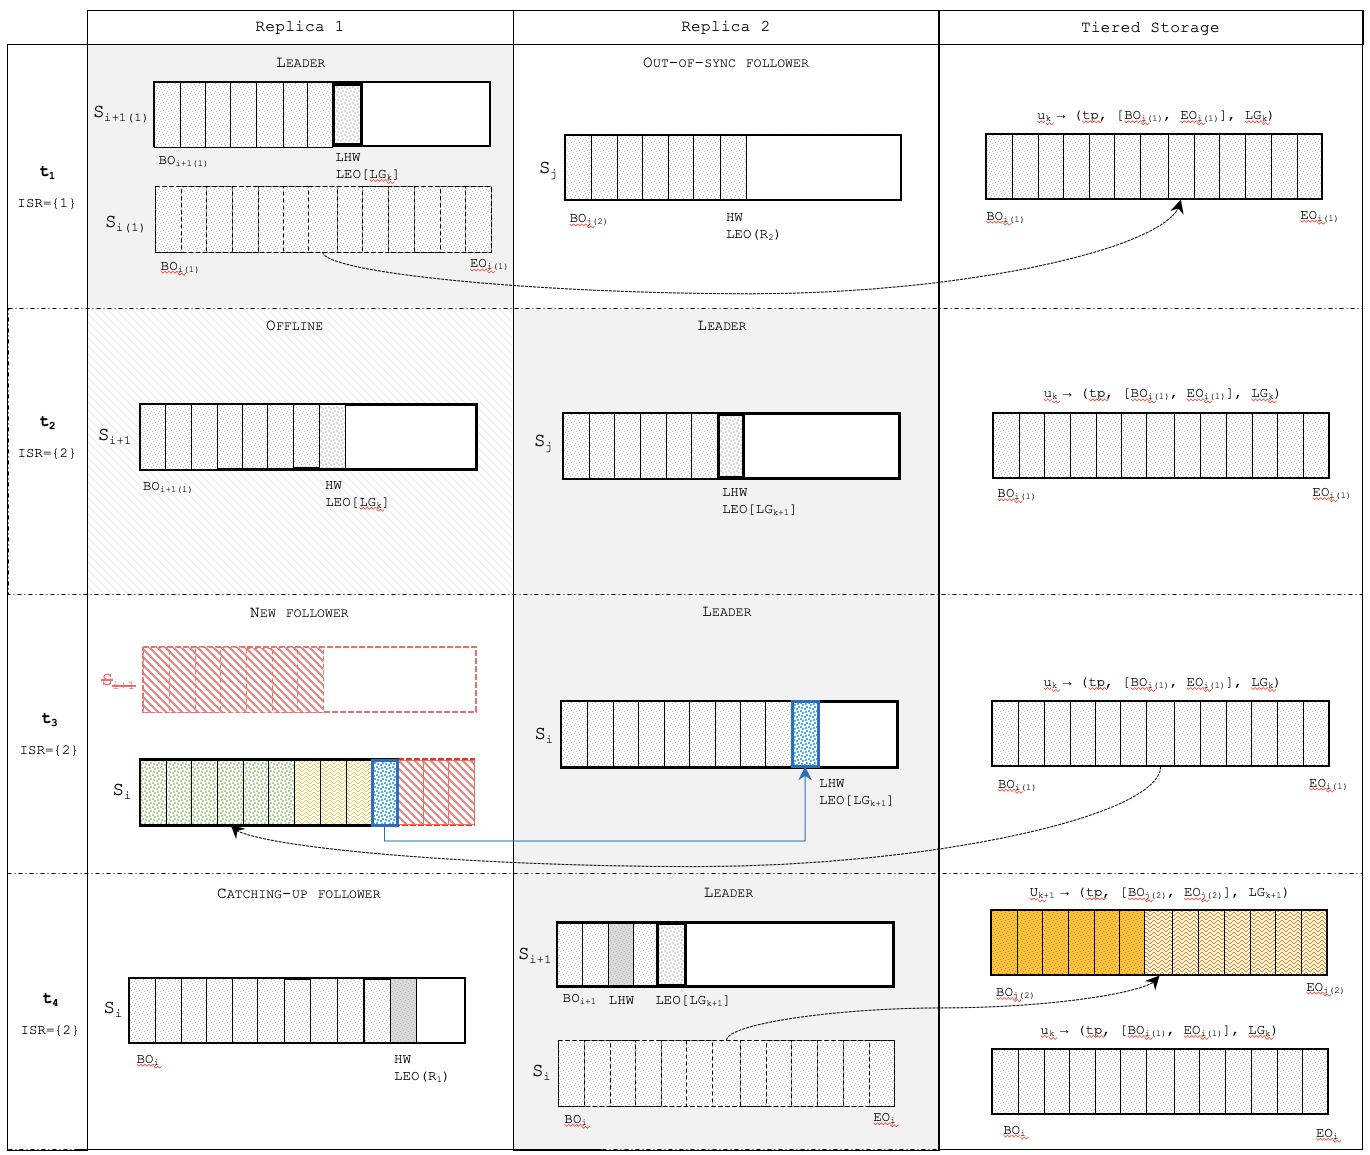
\includegraphics[scale=0.4]{img/unclean1.png}
	\captionof{figure}{Use of tiered segments to preserve local replica lineage.}
	\label{fig:simple-example}
\end{figure}

\begin{figure}[h!]
	\centering
	\renewcommand{\arraystretch}{2} % Default value: 1
	\begin{tabular}{|c|c|c|c|c|c|c|c|}
		\hline
		 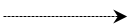
\includegraphics[scale=0.4]{img/offload.png}  & 
\includegraphics[scale=0.4]{img/onload.png} & 
\includegraphics[scale=0.4]{img/fetch.png} &  
\includegraphics[scale=0.4]{img/restored.png} & 
\includegraphics[scale=0.4]{img/divergent.png} & 
\includegraphics[scale=0.4]{img/duplicated.png} & 
\includegraphics[scale=0.4]{img/truncated.png} &  
\includegraphics[scale=0.4]{img/fetch record.png} \\
		 \hline
		Offload & Onload & Fetch & Reinstated & Divergent & Duplicated & Truncated & Fetch source/target \\
		\hline
	\end{tabular}
	\captionof{figure}{Legend}
\end{figure}

\subsection{Divergent remote replica lineage}

Shoud the segments $S(u_k)$ and $S(u_{k+1})$ be reconciled? One of them deleted? 

\subsubsection{Lineage reconstruction}

Let us consider this follow-up use case, where a third replica is added to the previous example. This replica shares the same lineage as replica 1 up to generation $k$, then becomes offline at the same time as replica 1. It comes back online long after the latter, and replica 2 has produced segments $S_j^2$, $S_{j+1}^2$ and $S_{j+2}^2$. Assume $S_i^1$ is replicated by $S_i^3$ in replica 3, and that the latter is not available locally as it was deleted based on log retention policies. Replica 3 should follow the same replication steps as replica 1 to construct its lineage post-generation $k$, which means, truncating and replicating from replica 2.

The problem is segments $S_j^2$, $S_{j+1}^2$ and $S_{j+2}^2$ may be tiered and not available locally. That means that, to reconstruct its lineage, replica 3 would require replication of segments from the tiered storage. One could argue that replica 3 could borrow the same lineage as replica 1. However, nothing guarantees lineage has not diverged after generation $k$. To illustrate this, imagine that before replica 3 is back online, replica 2 goes offline and replica 1 takes back leadership, ingests some records beyond $LEO_{k+1}$, then goes offline again, then replica 2 comes back and re-acquire leadership and resume ingesting. Should all segments be local, replica 3 would not inquire about replica 1 and simply replicates replica 2 from $min(LEO_{k}^3, LEO_{k+3}^2)$. The lineage of replica 3 should derive from the current leader at the current generation.

\subsubsection{Non-evictability of remote segments}

Evicting segments from the tiered storage for any of the replica lineage is not always decidable \textit{a priori}. Consider the scenario where a topic-partition has three replicas, one of which $\mathcal{R}_3$ has been offline for a month due to a misconfiguration. During a maintenance operation, the two "healthy" replicas $\mathcal{R}_1$ and $\mathcal{R}_2$ are put offline and $\mathcal{R}_3$ brought back online, empty. Unclean leader election is enabled and $\mathcal{R}_3$ becomes the leader of the topic-partition for the generation $g$. How to decide if the one-month worth of data of the "healthy" replicas should be preserved?

Let us consider the two distinct use cases below.

\begin{outline}[enumerate]
	\1 In the first case, the $\mathcal{R}_1$ and $\mathcal{R}_2$ come back online and become follower of $\mathcal{R}_3$. Local segments are truncated and data above $LEO_g$ are discarded.
	\1 In the second case,  $\mathcal{R}_3$ goes back offline shortly after and before $\mathcal{R}_1$ and $\mathcal{R}_2$ comes back alive. Pre-maintenance lineage is preserved.  
\end{outline}

As a result, whether or not tiered segments can be evicted is not decidable if lineage divergence is allowed, because to preserve equivalence, these segments may be required for future generations.
Note that in the first case, the tiered storage would preserve the segments unlike the local storage. The durability guarantees when tiered storage is enabled should be stronger, not weaker, than with a local storage only.

More formally, if $k$ is the tier of the storage layer (for instance, tier 0 = ephemeral storage, tier 1 = log directory and tier 2 = remote storage), for a given record $r$ decided at $t_0$, the probability of a successful read of that record at a time $t_1 > t_0$ should observe
\[
P_{k+1}(r, \Delta t) \geq P_{k}(r, \Delta t), \Delta t = t_1 - t_0
\] 

\section{Misaligned base offsets}

It is possible that base offsets of the segments of distinct replicas do not match, even when these replicas are in sync. This can be for instance be a consequence of a previous unclean leader election. Such cases need to be handled gracefully by the tiered storage, which should allow duplicated offset of non-divergent lineages.

\subsubsection{Left offsets overlap}

Consider the example provided in Figure \ref{fig:left-overlap}. A topic-partition is comprised of two replicas. 

\begin{outline}[enumerate]
	\1 At $t_1$, generation $k$, replica 1 is the leader and segment $S_i^1$ is offloaded successfully and its active segment is $S_{i+1}^1$ starting at $BO_{j+1}^1$. Replica 2 is in sync with the leader. Its active segment $S_j^2$ starts at offset $BO_j^2$ which is slightly behind $BO_{j+1}^1$. 
	\1 Leadership is switched between replica 1 and 2 at generation $k+1$ as a result of an admistrator operation. Replica 2 ingests records and at some point $S_j^2$ is offloaded. There is an overlap of offsets for the range $[BO_j^2..EO_i^1]$, but this should not prevent $S_j^2$ to be offloaded.
	\1 A consumer starts polling for records from the leader of the topic-partition with a fetch offset equals to $BO_i^1$. The leader retrieves the segment $S(u_k)$ from the tiered storage and starts reading from the segment, responding to fetch requests with that segment until $EO_i^1$ is reached. At this point, the segment $S(u_{k+1})$ is used, but records in the offset range $[BO_j^2..EO_i^1]$ are skipped. 
\end{outline}

\subsubsection{Right offsets overlap}

This is illustrated in Figure \ref{fig:right-overlap} with a slightly different scenario exhibiting the same method.

\begin{outline}[enumerate]
	\1 The same misalignment of base offsets as in the previous example is observed. This time, $S_i^1$ is not offloaded successfully because of the tranisent unavailability of the tiered storage.
	\1 Replica 1 goes offline and leadership is assigned to replica 2 which is in sync with replica 1 at the time of the event. Records are ingested and $S_j^2$ is offloaded successfully.
	\1 Replica 1 comes back online and replicates from 2. At some point the segment $S_i^1$ is rolled over and become eligible for tiering. Since some records, starting at offset $BO_i^1$, have not been tiered. \textbf{However, in the current design, segments can only be offloaded by the leader}. What to do here? If replica 1 never acquires leadership again, and is not fetched from as a preferred read replica, the records missing from $S_j^2$ will never be promoted for tiering, thus weakening the durability re-inforcement provided by the usage of tier storage (though not the tier storage itself), should the local $S_j^2$ be lost afterwards. 
\end{outline}

Note that misaligned base offsets can result from unclean leader election.

TODO: is unclean leader election necessary for base offset misalignment to happen?

TODO: Evaluate the impact of a) compressed record batches b) transactions

The algorithm which results depends on whether a given fetch request satisfied from tiered segments support cross-segment reads, that is, reading from two consecutive segments. 

\begin{figure}[h!]
	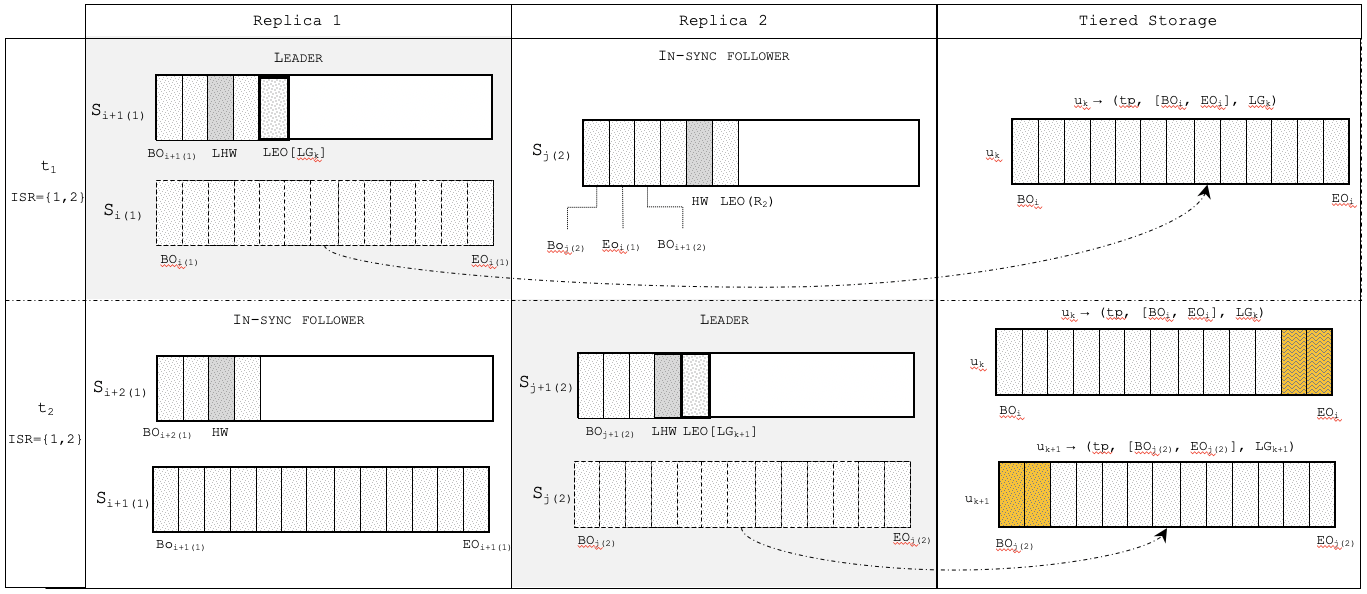
\includegraphics[scale=0.4]{img/left-overlap.png}
	\captionof{figure}{Left-overlap in tiered storage as a result of base offset misalignment.}
	\label{fig:left-overlap}
\end{figure}

\begin{figure}[h!]
	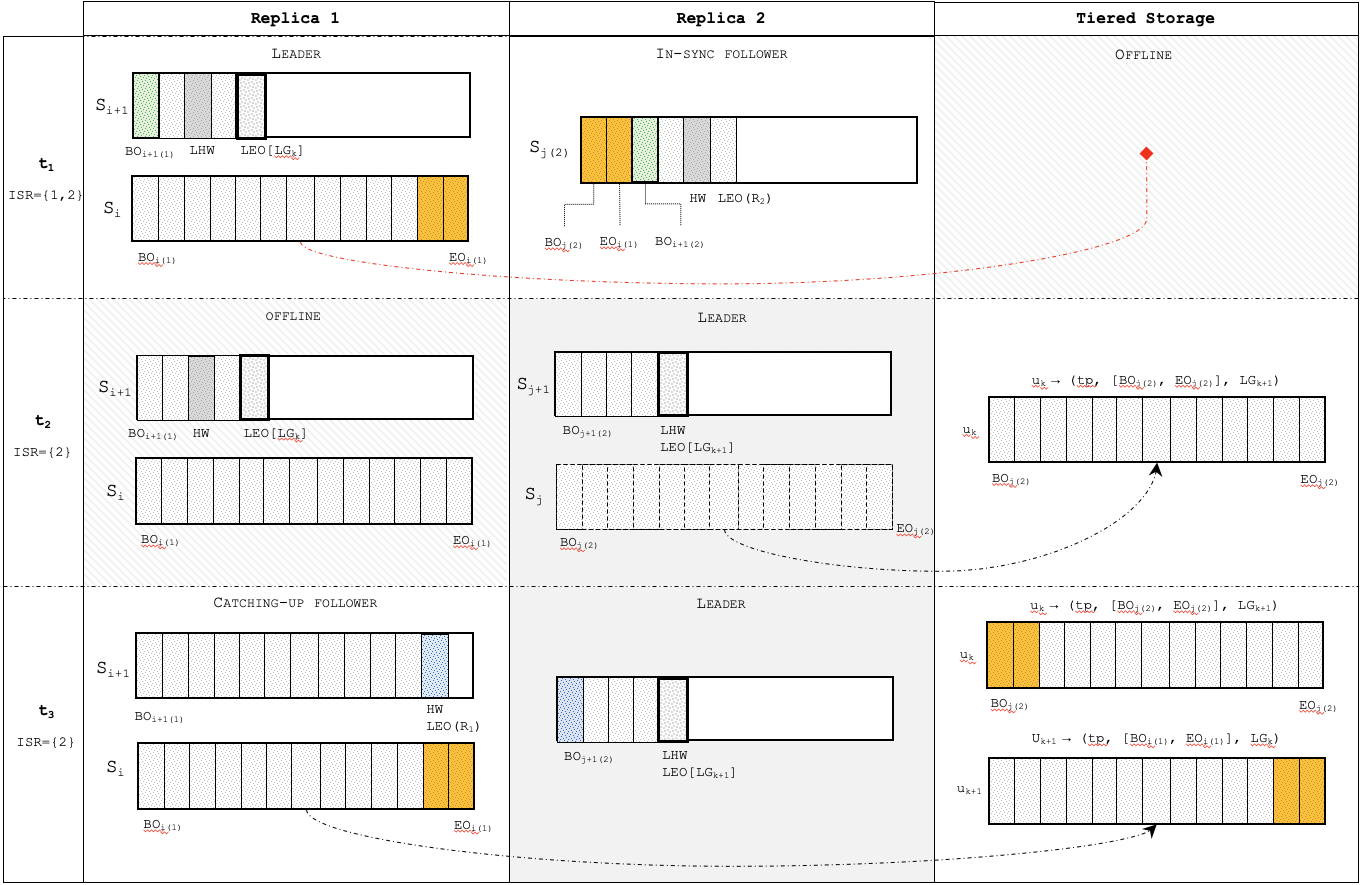
\includegraphics[scale=0.4]{img/right-overlap.png}
	\captionof{figure}{Right-overlap in tiered storage as a result of base offset misalignment.}
	\label{fig:right-overlap}
\end{figure}

\end{document}
